%
% transport.tex -- Animation Paralleltransport
%
% (c) 2021 Prof Dr Andreas Müller, OST Ostschweizer Fachhochschule
%
\bgroup
\definecolor{darkred}{rgb}{0.8,0,0}
\begin{frame}[t]
\setlength{\abovedisplayskip}{5pt}
\setlength{\belowdisplayskip}{5pt}
\frametitle{Paralleltransport}
\begin{center}
\begin{tikzpicture}[>=latex,thick]
\uncover<1>{
\node at (0,0) {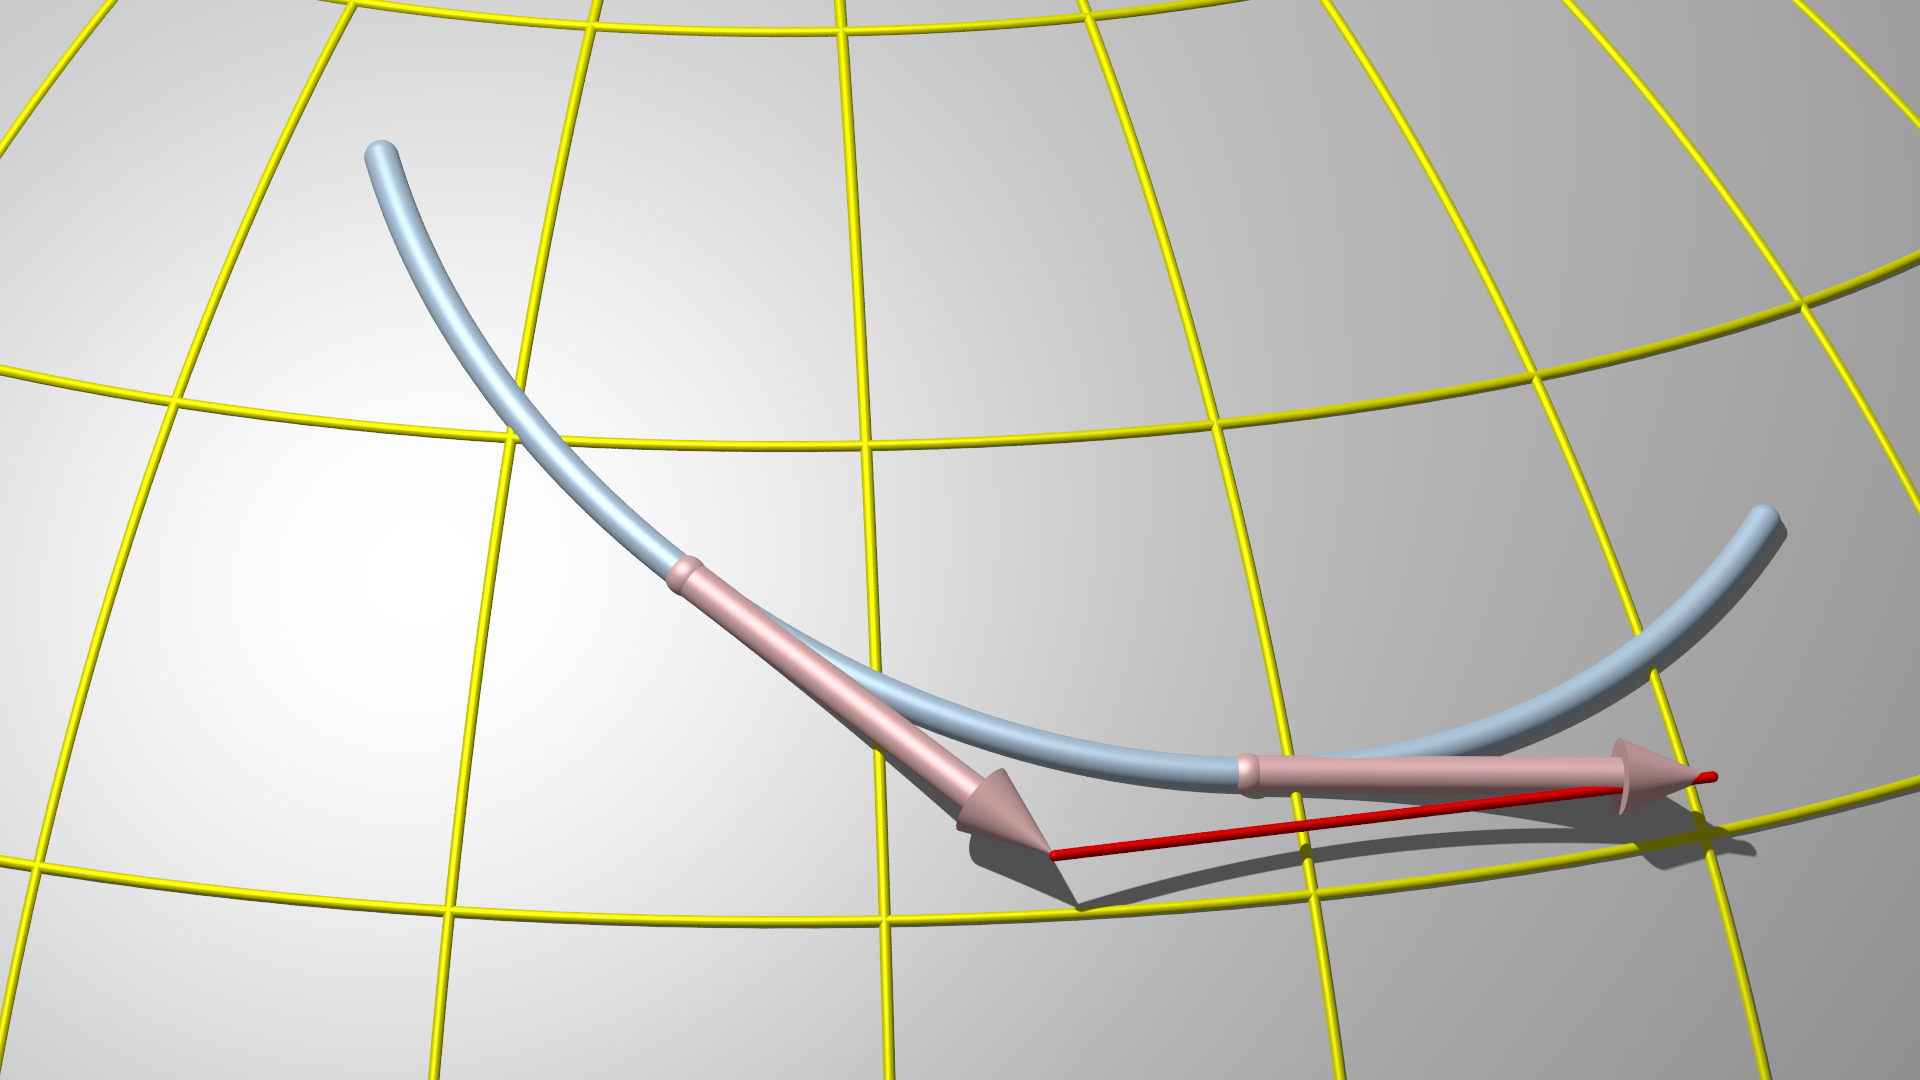
\includegraphics[width=12cm]{../slides/7/differenz.jpg}};
\node at (-2.2,-0.5) {$\gamma(t)$};
\node[color=white] at (0.4,-2.2) {$\dot{\gamma}(t)$};
\node at (1.9,-1.1) {$\gamma(t+\Delta t)$};
\node[color=white] at (4.9,-1.9) {$\dot{\gamma}(t+\Delta t)$};
\node[color=darkred] at (2.5,-2.1) [scale=1.5] {?};
}
\uncover<2>{
\node at (0,0) {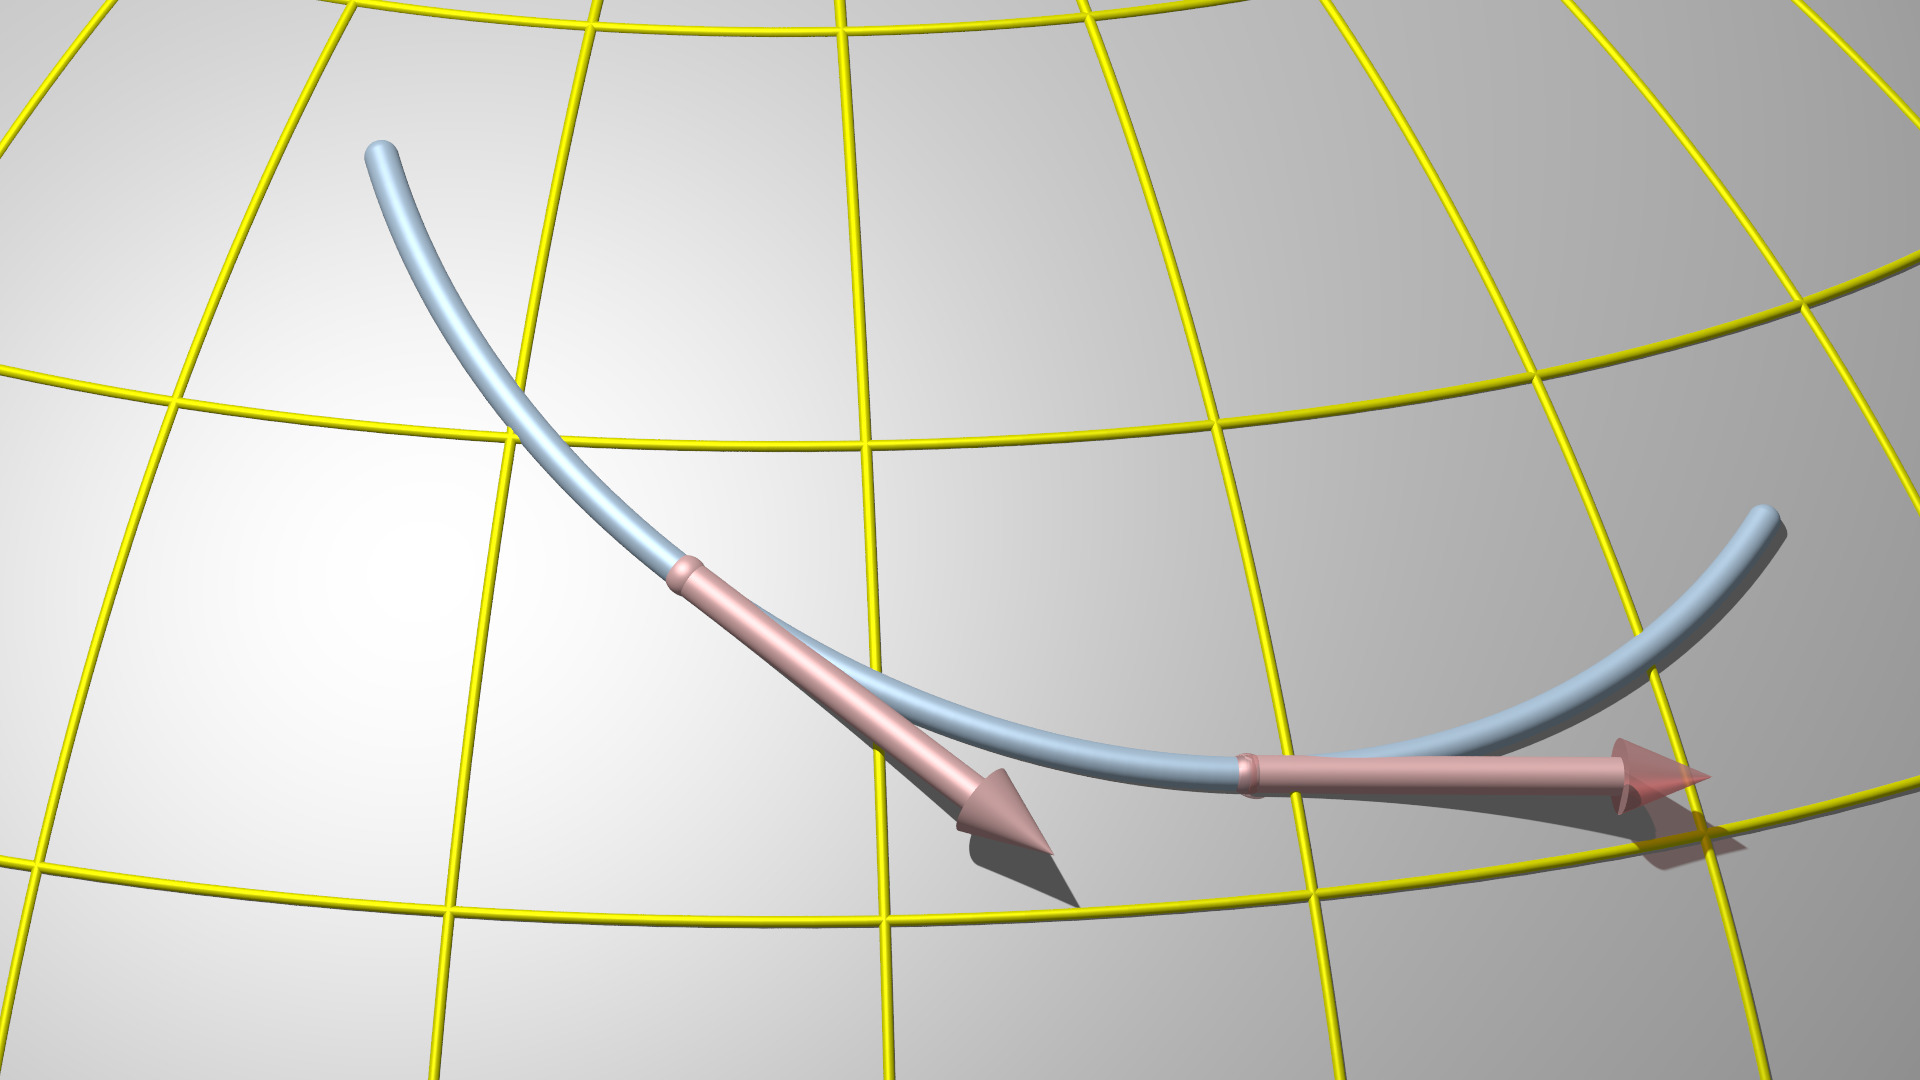
\includegraphics[width=12cm]{../slides/7/d01.jpg}};
}
\uncover<3>{
\node at (0,0) {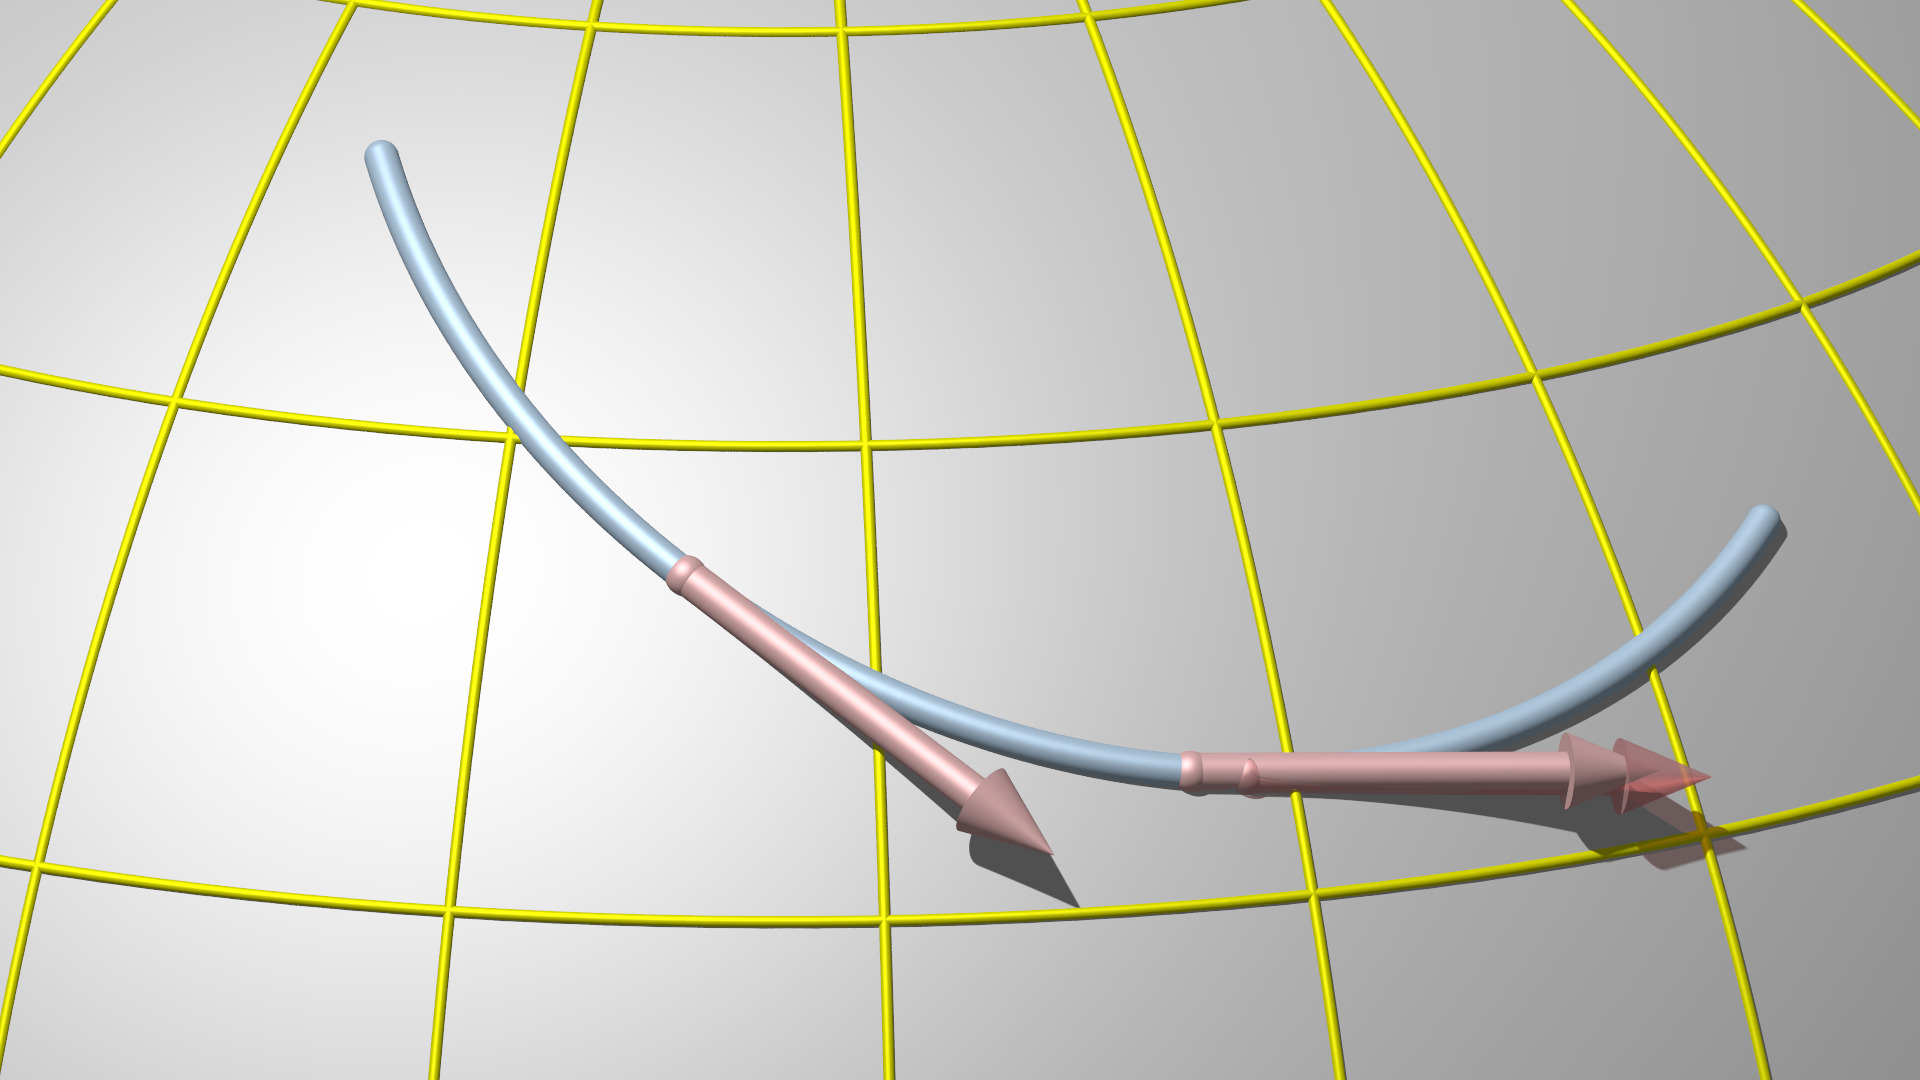
\includegraphics[width=12cm]{../slides/7/d02.jpg}};
}
\uncover<4>{
\node at (0,0) {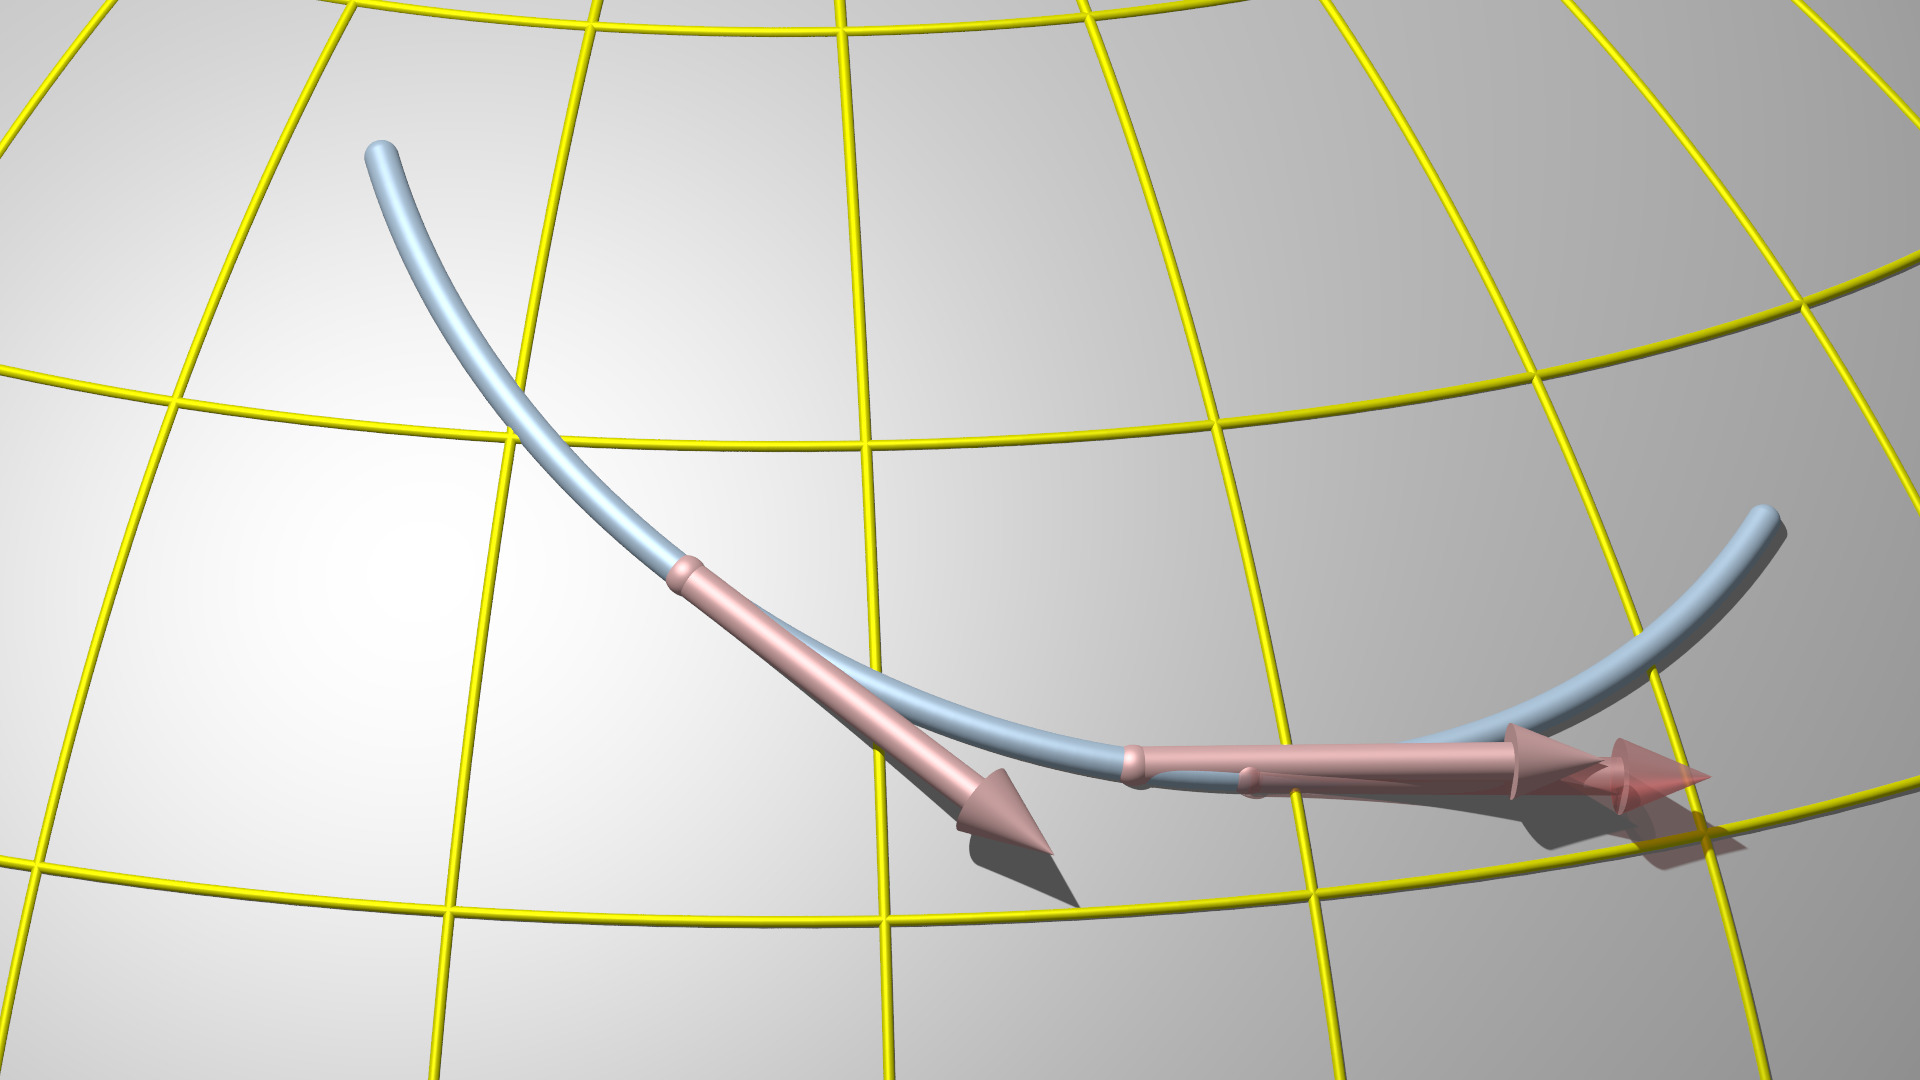
\includegraphics[width=12cm]{../slides/7/d03.jpg}};
}
\uncover<5>{
\node at (0,0) {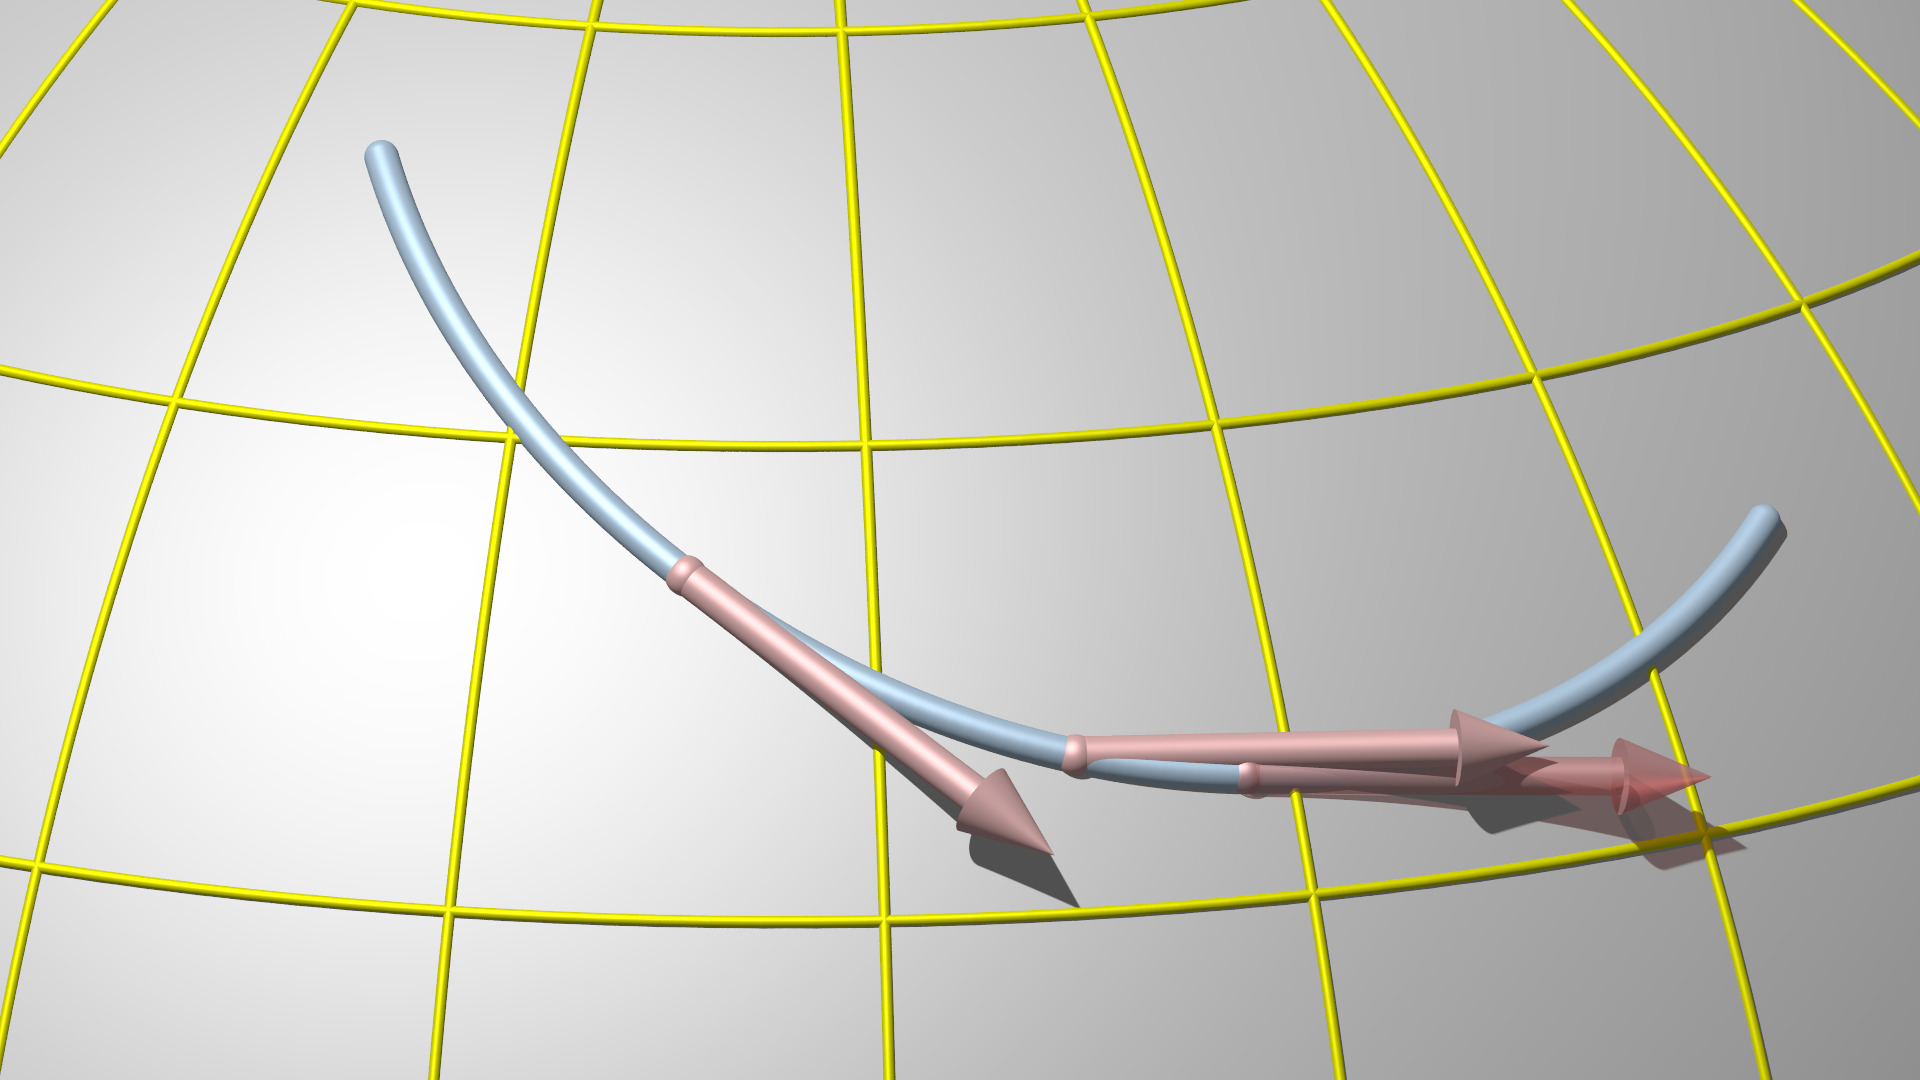
\includegraphics[width=12cm]{../slides/7/d04.jpg}};
}
\uncover<6>{
\node at (0,0) {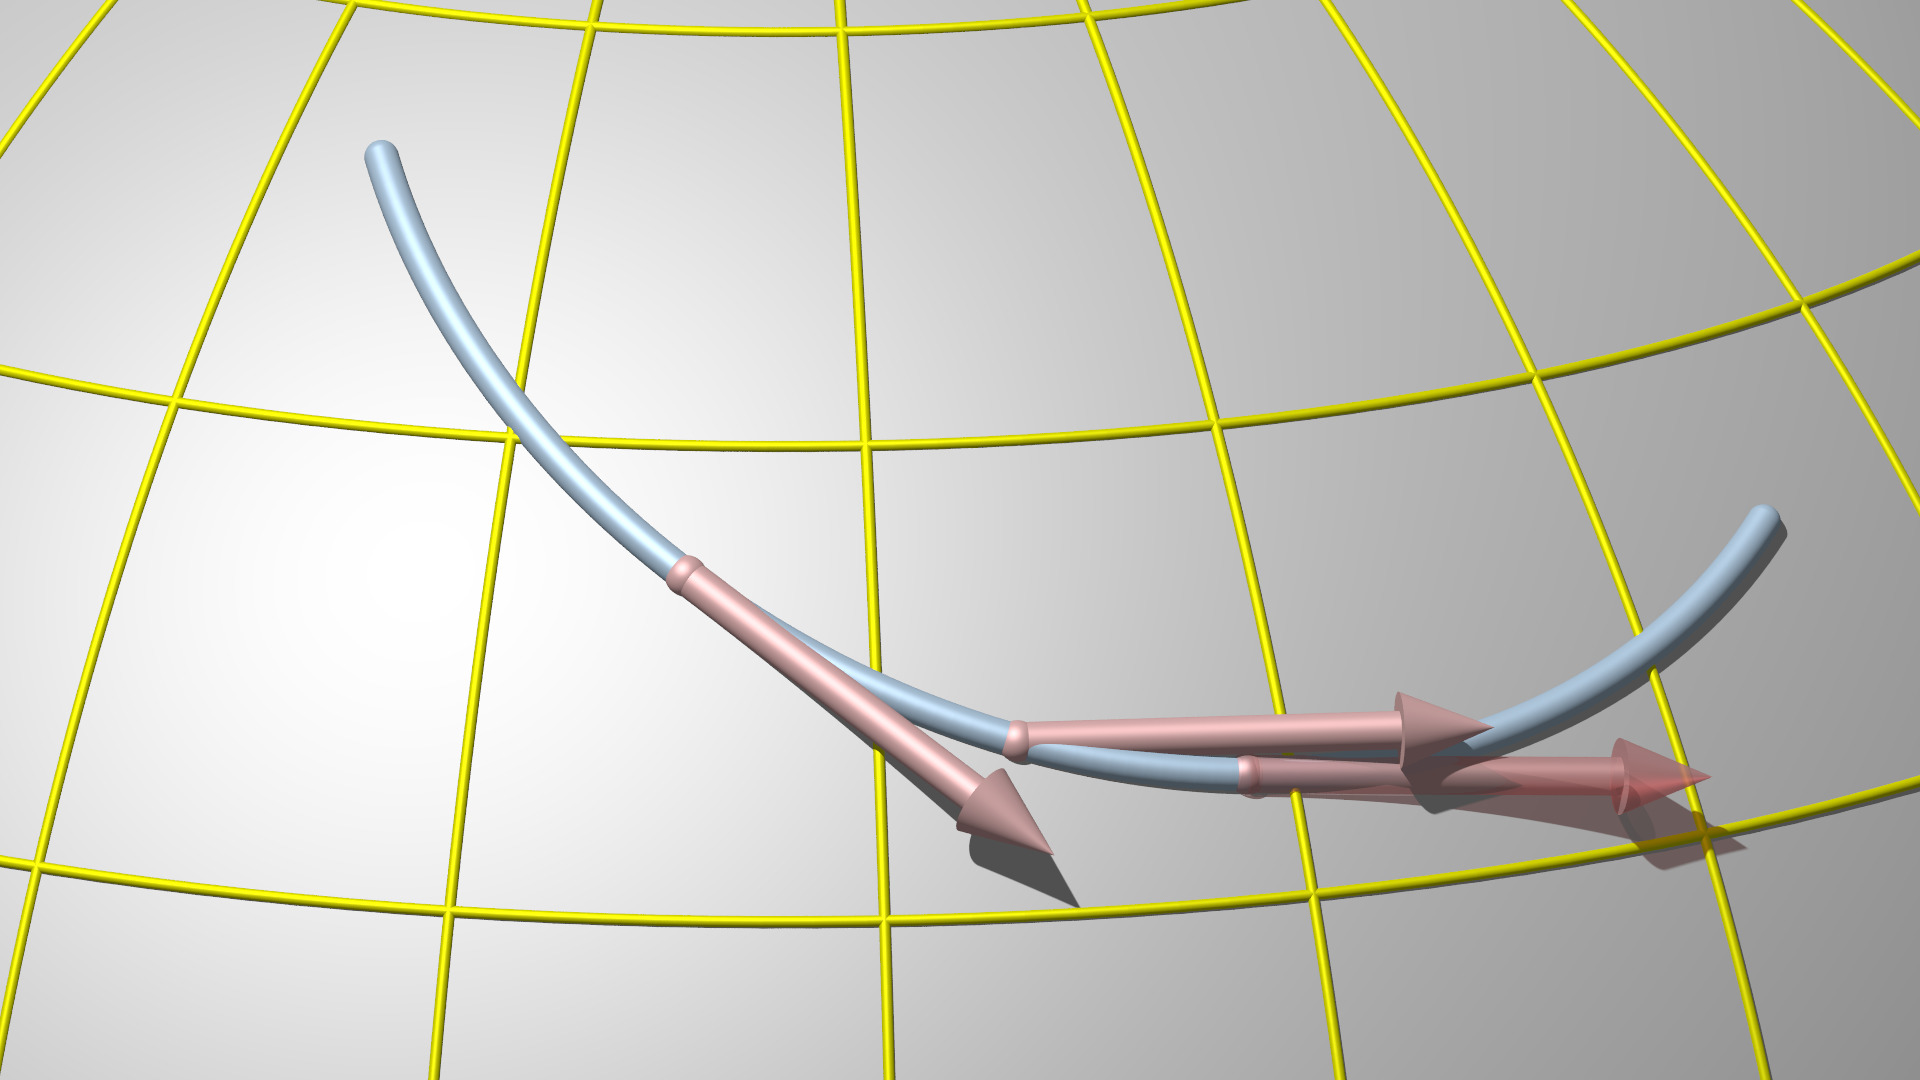
\includegraphics[width=12cm]{../slides/7/d05.jpg}};
}
\uncover<7>{
\node at (0,0) {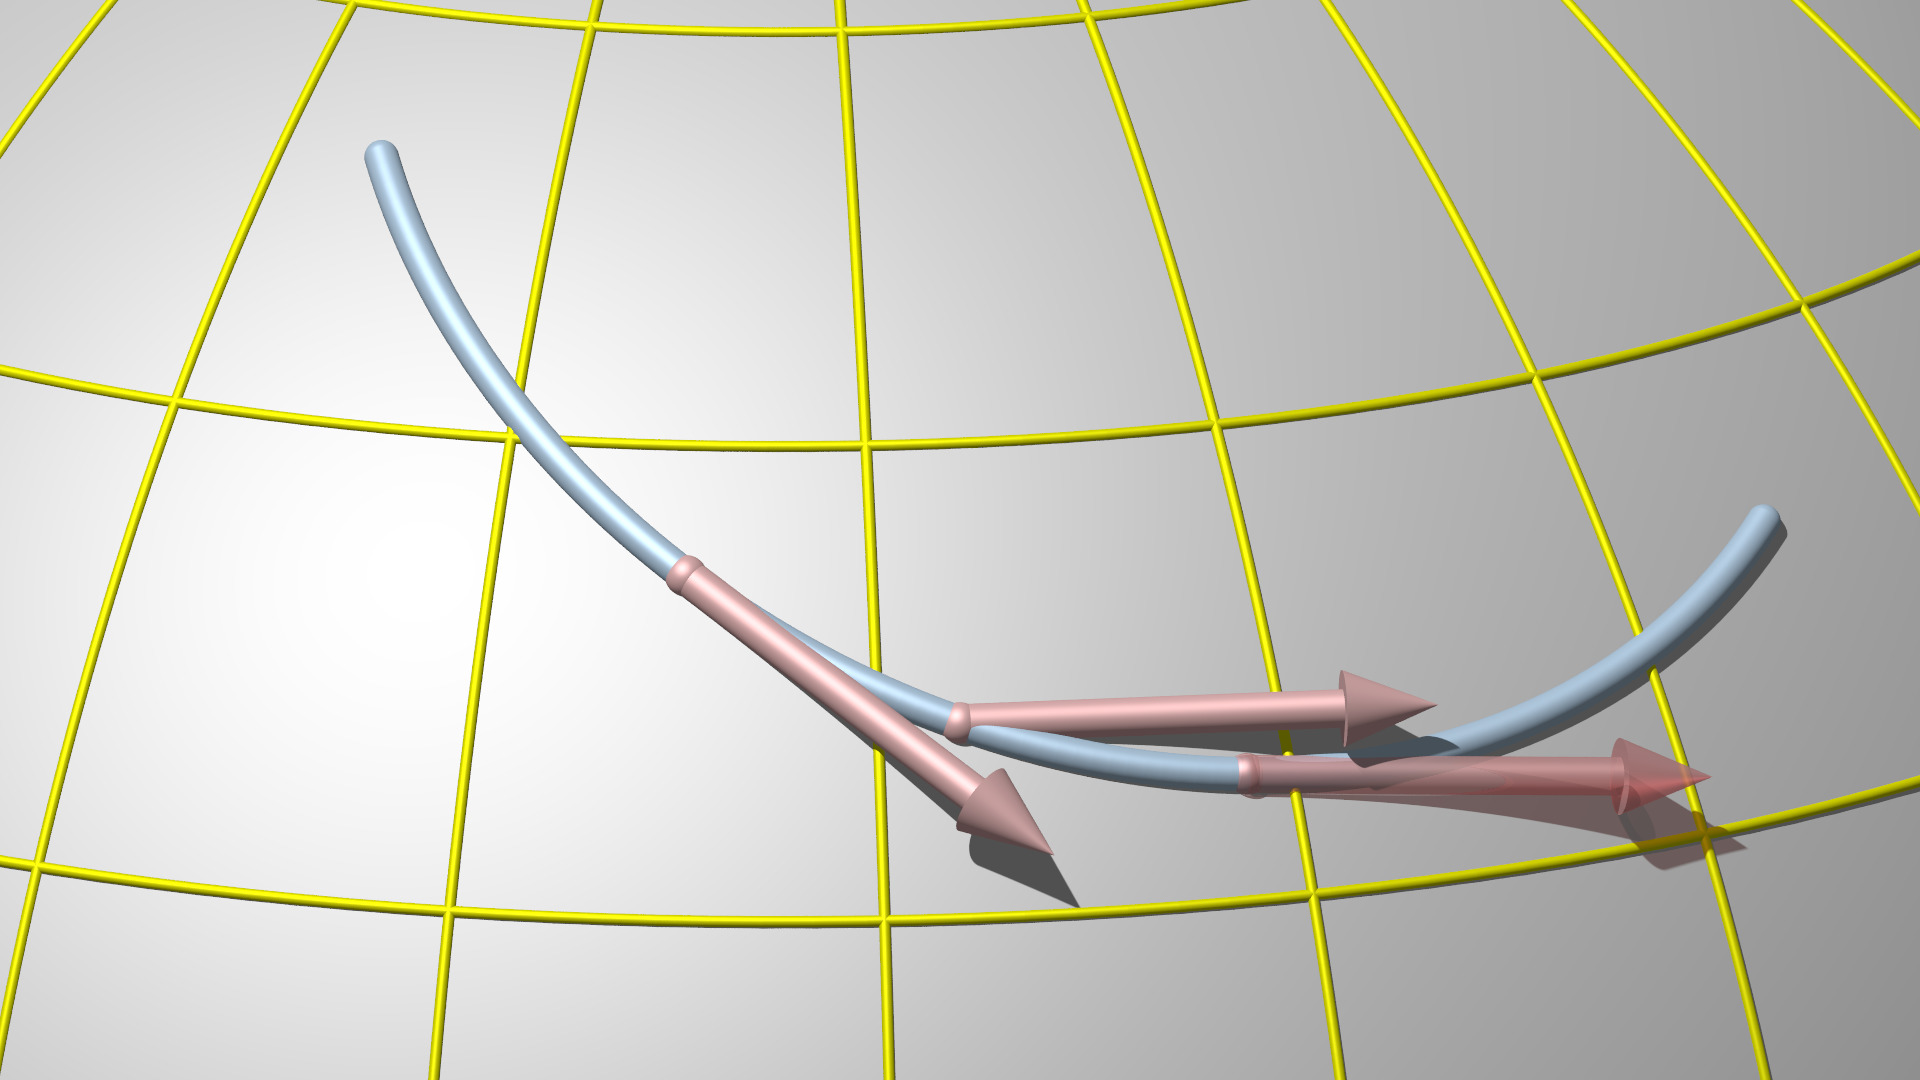
\includegraphics[width=12cm]{../slides/7/d06.jpg}};
}
\uncover<8>{
\node at (0,0) {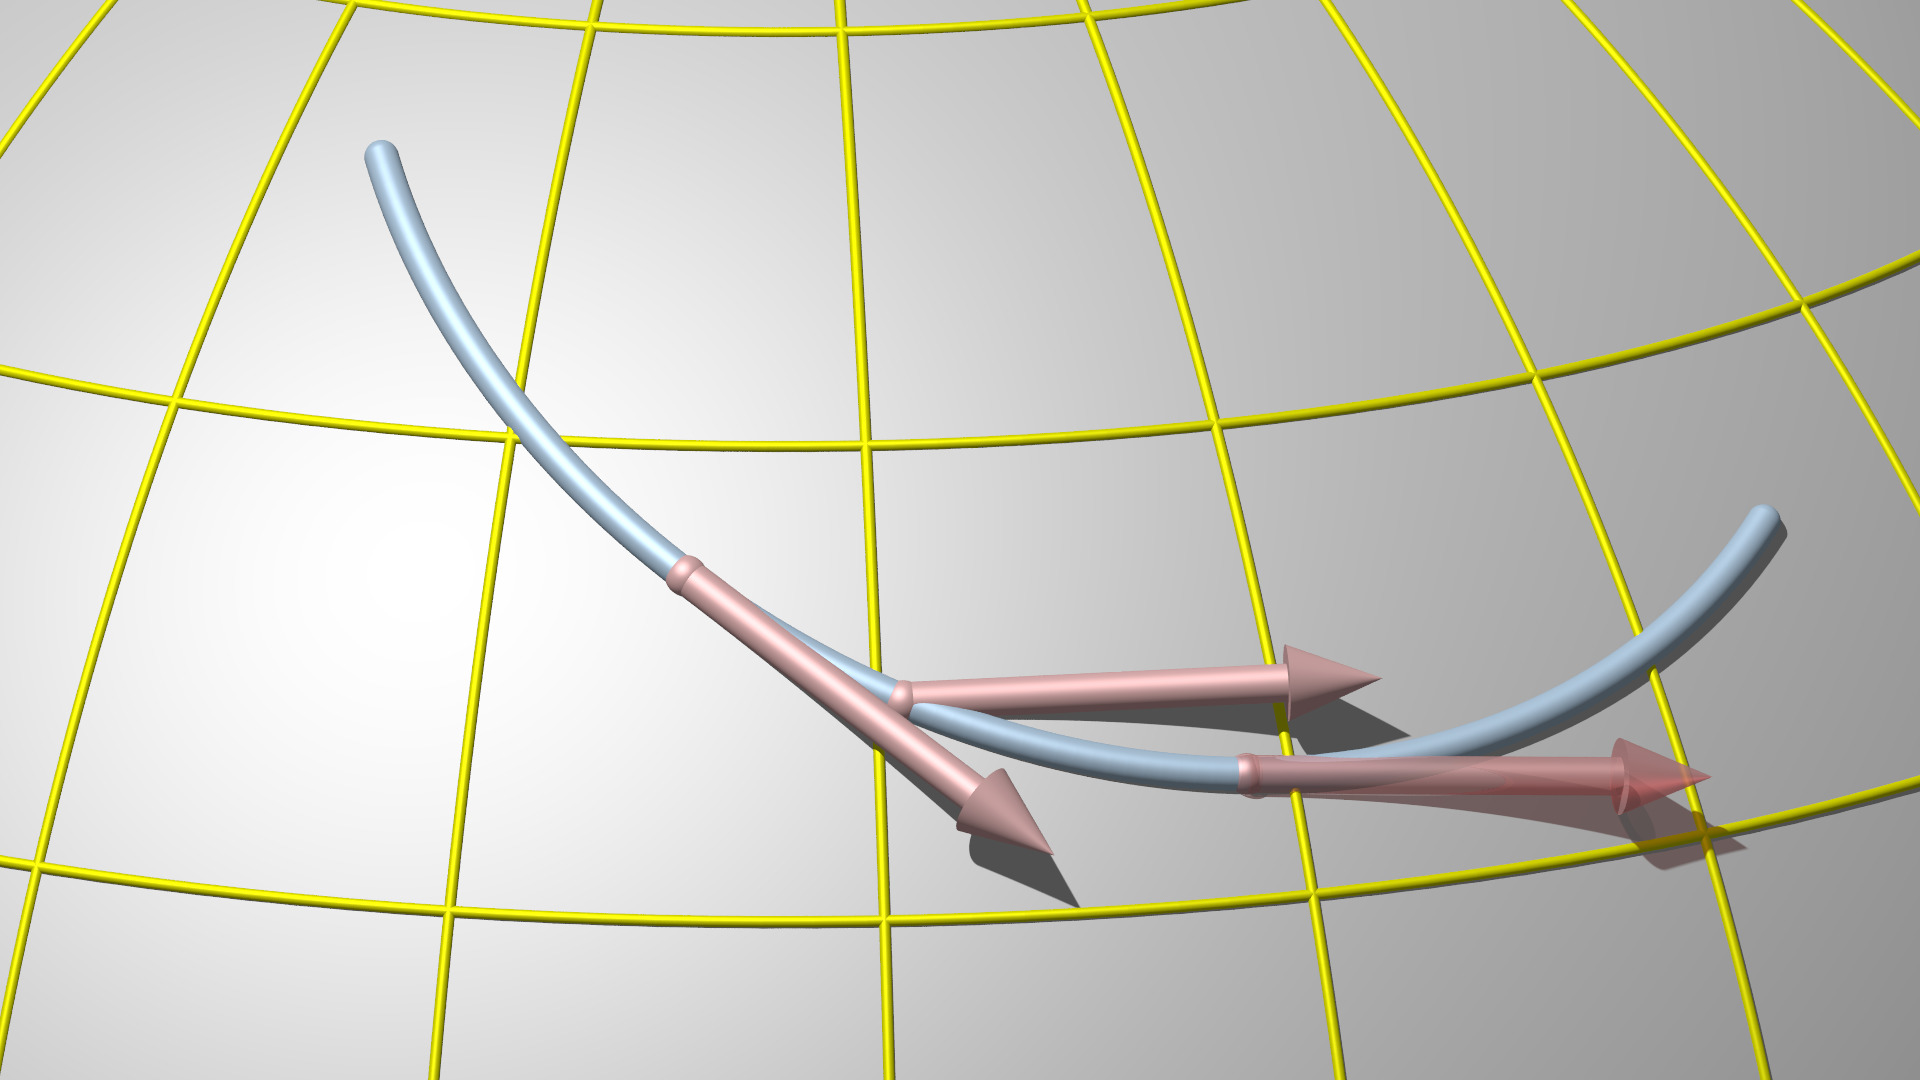
\includegraphics[width=12cm]{../slides/7/d07.jpg}};
}
\uncover<9>{
\node at (0,0) {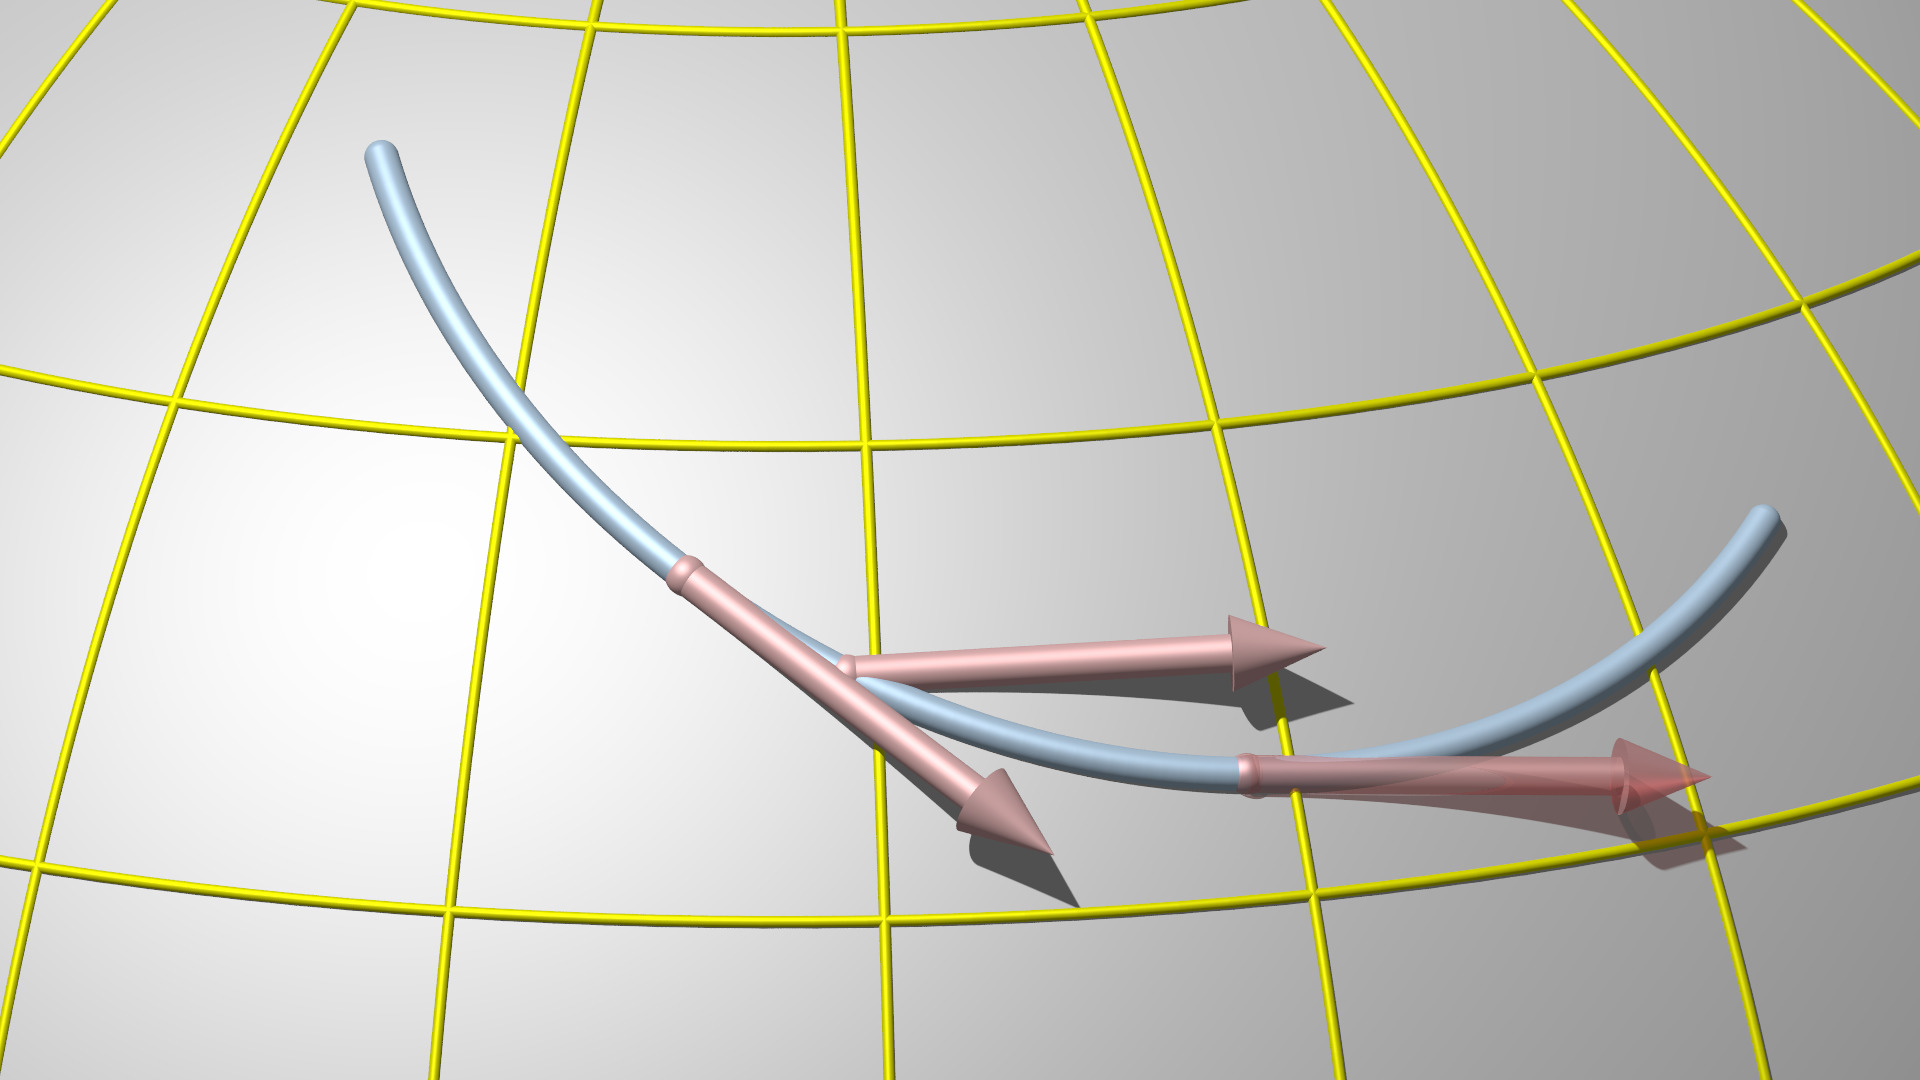
\includegraphics[width=12cm]{../slides/7/d08.jpg}};
}
\uncover<10>{
\node at (0,0) {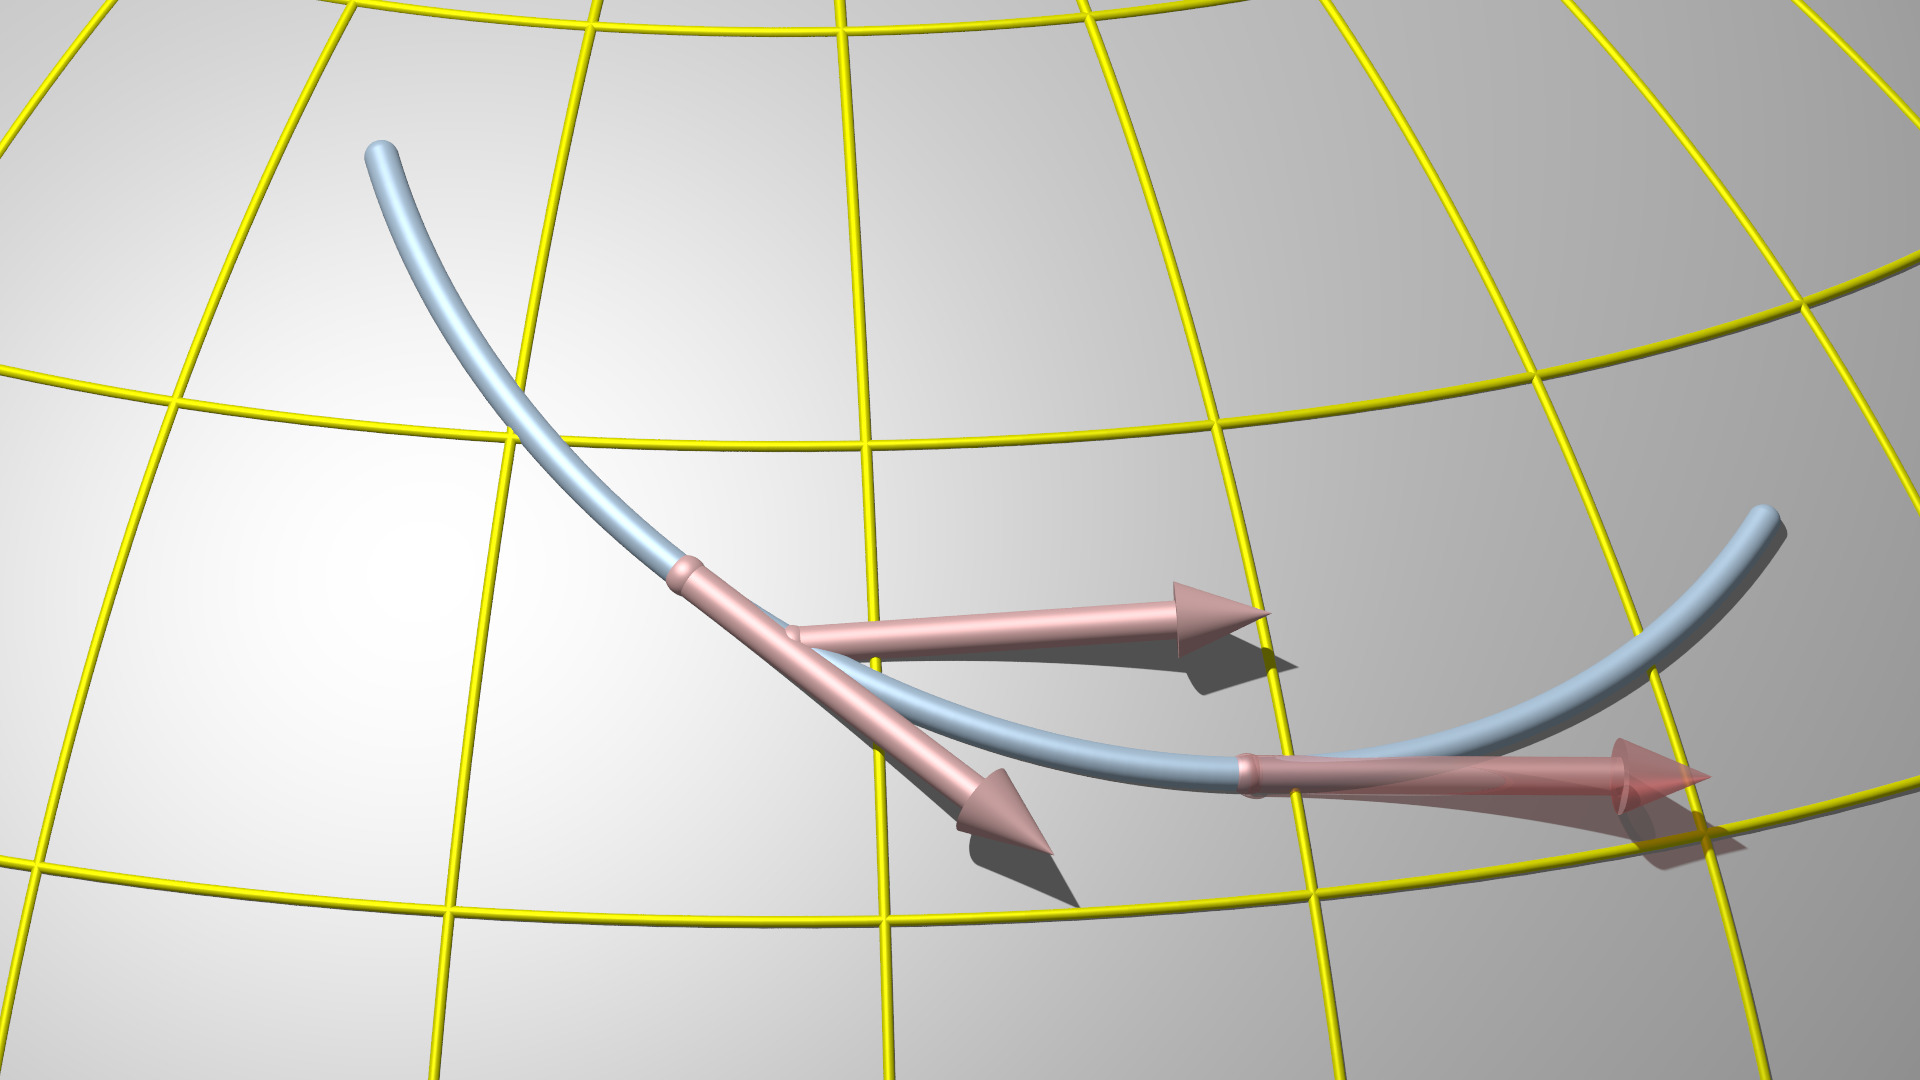
\includegraphics[width=12cm]{../slides/7/d09.jpg}};
}
\uncover<11>{
\node at (0,0) {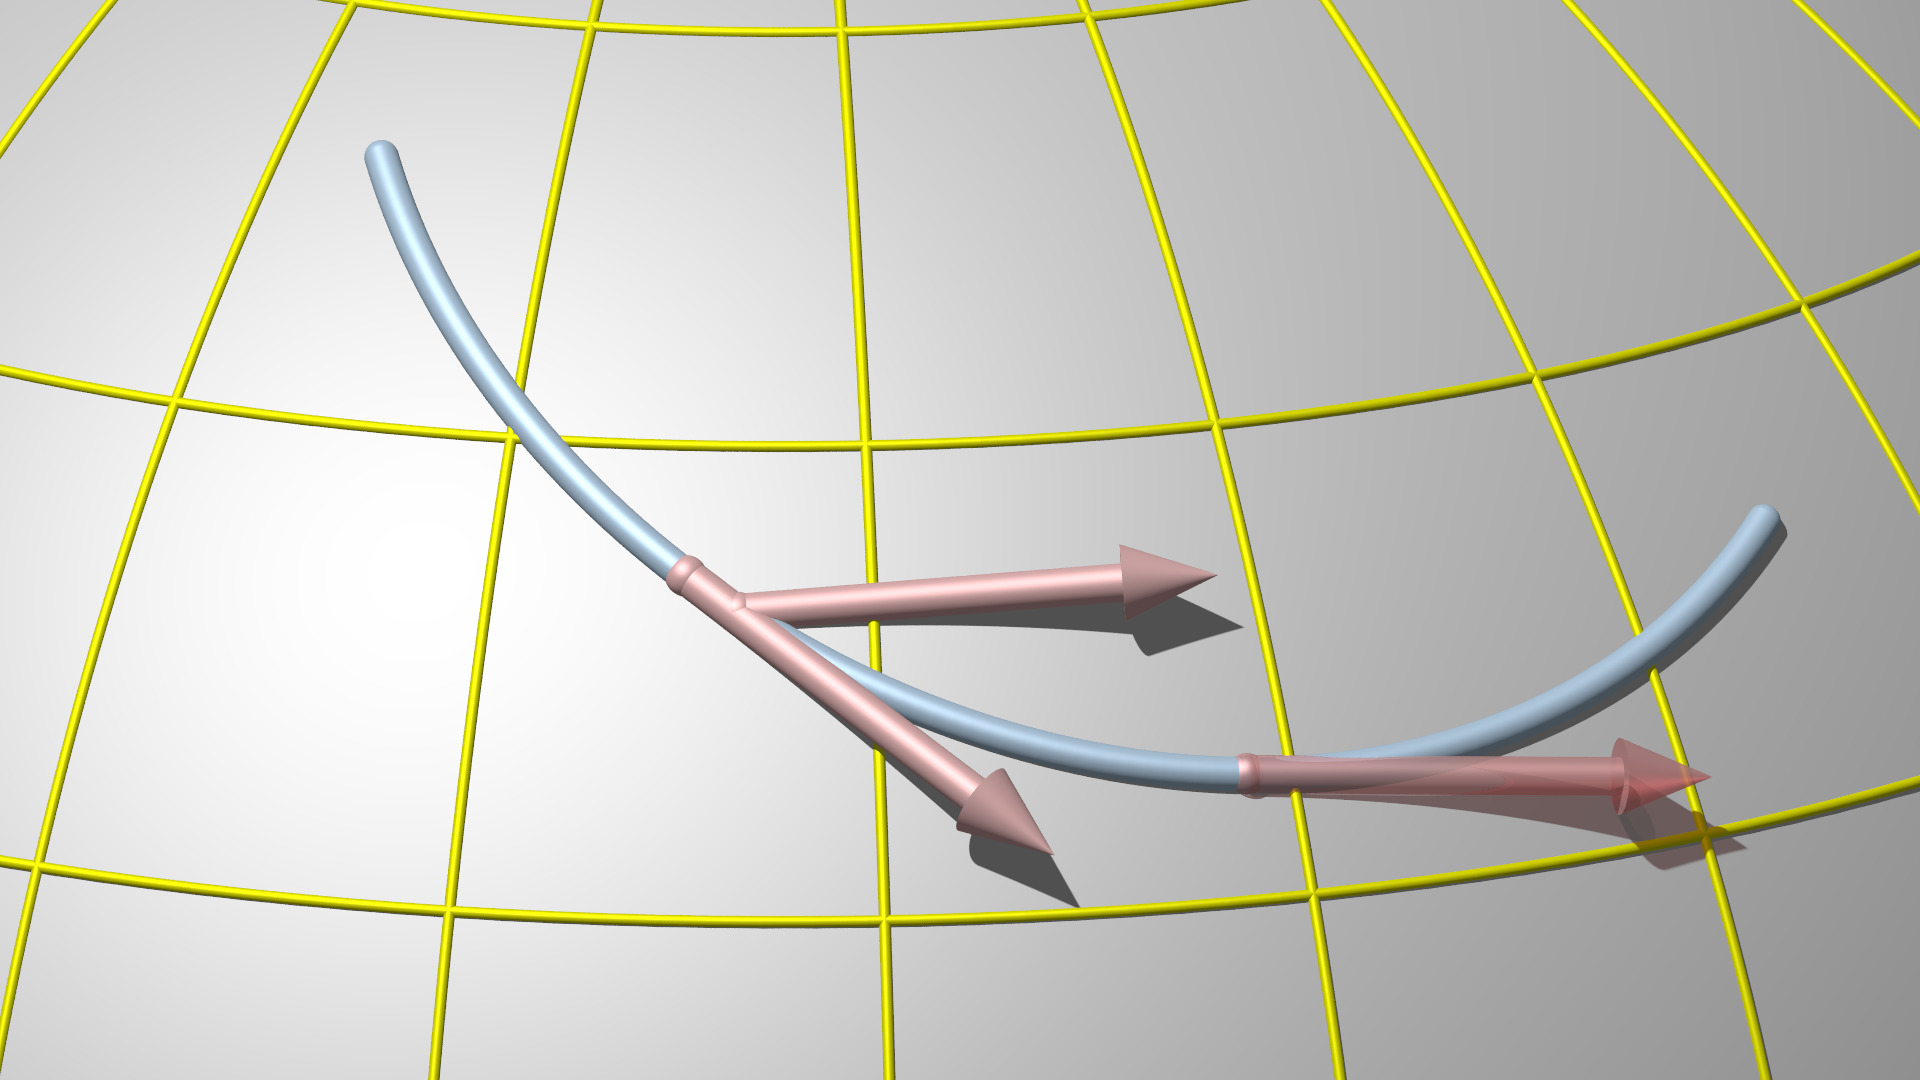
\includegraphics[width=12cm]{../slides/7/d10.jpg}};
}
\uncover<12>{
\node at (0,0) {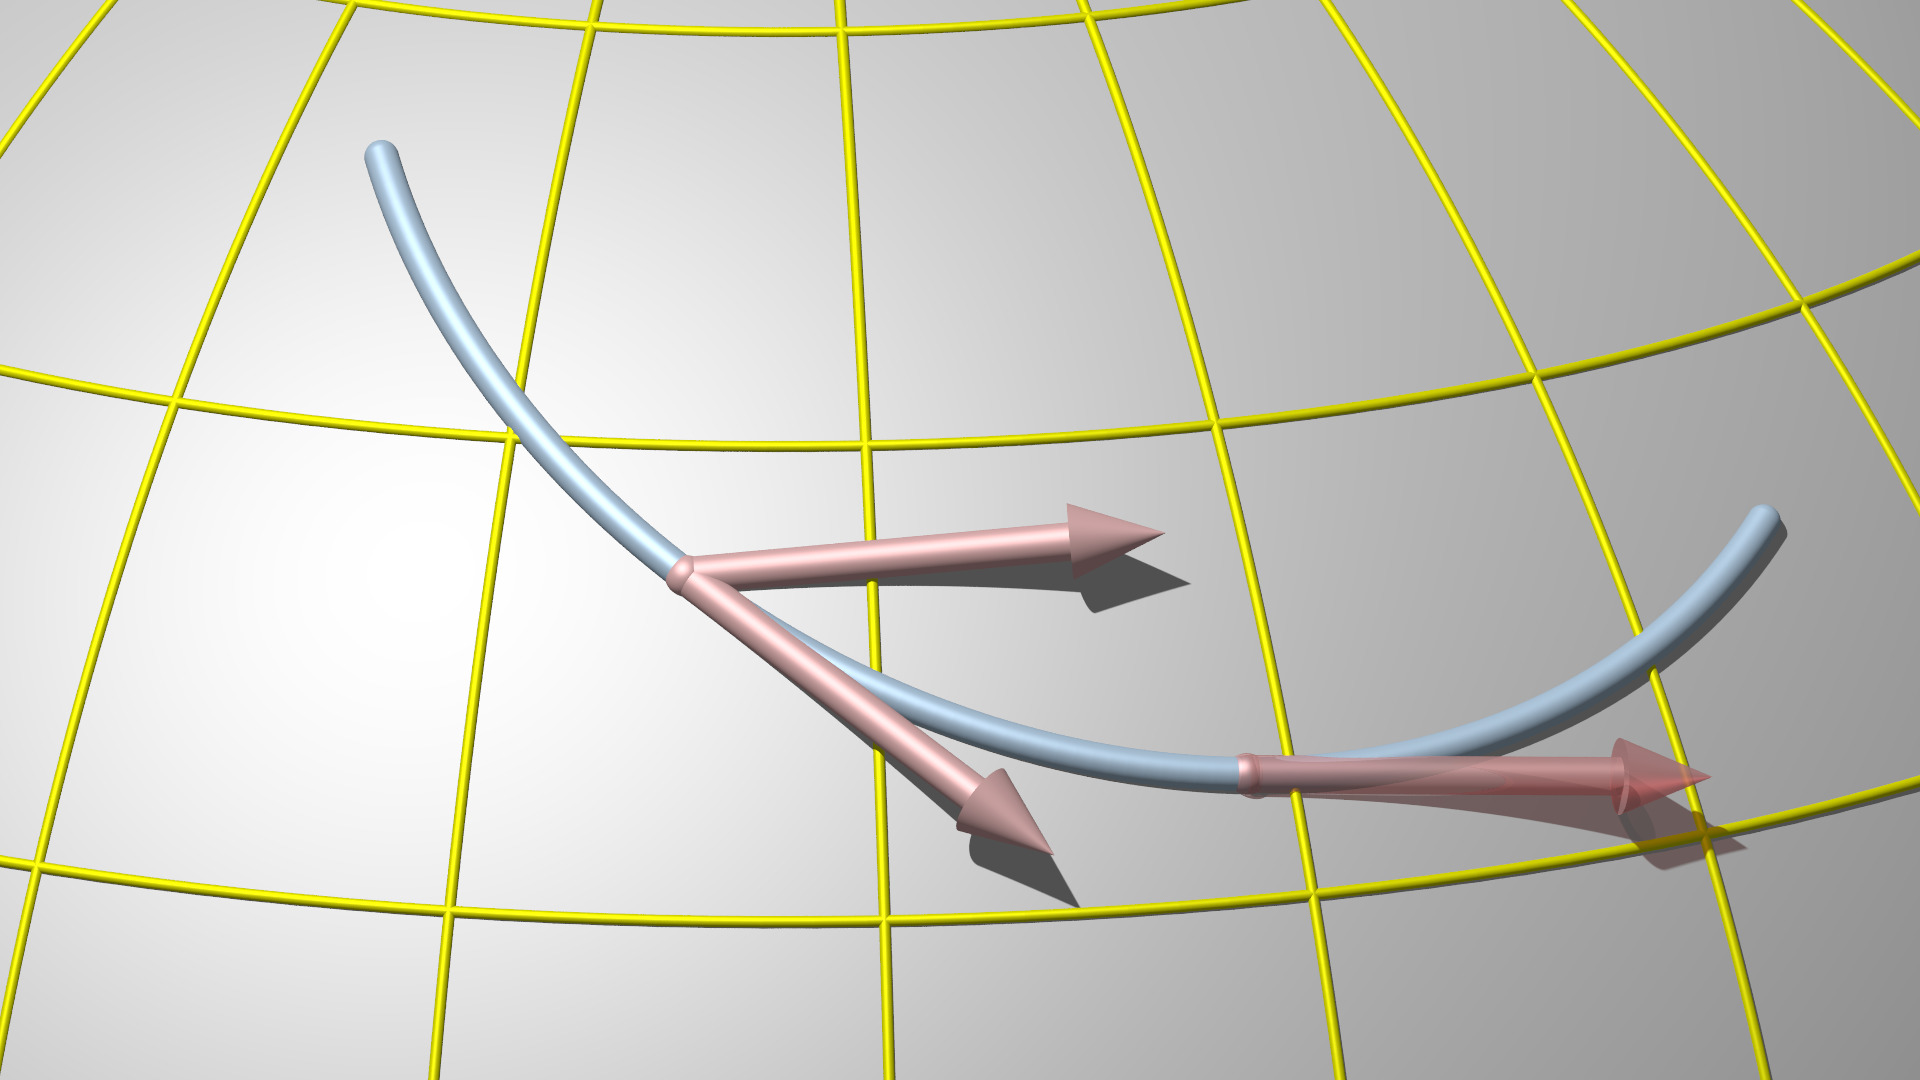
\includegraphics[width=12cm]{../slides/7/d11.jpg}};
}
\uncover<13>{
\node at (0,0) {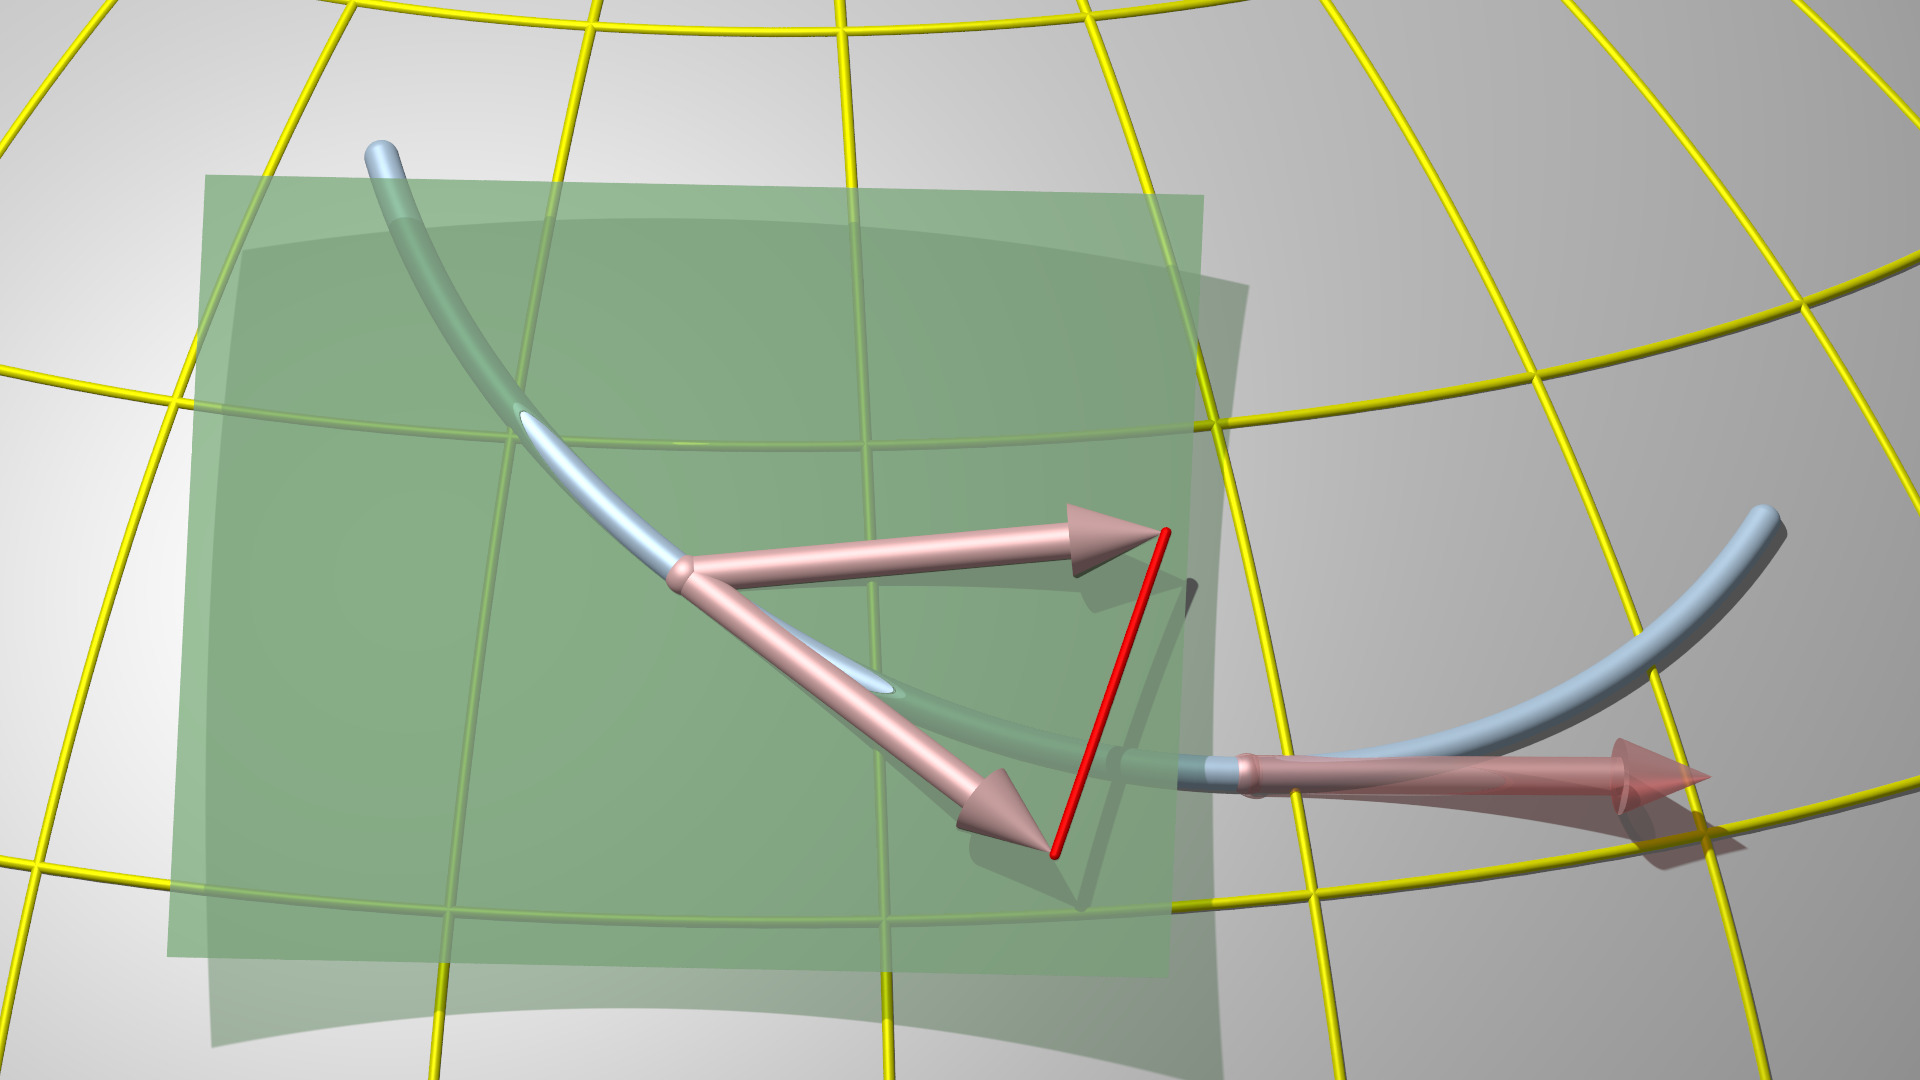
\includegraphics[width=12cm]{../slides/7/diffgedreht.jpg}};
\node at (0.7,1.7) {$T_{\gamma(t)}M$};
\node at (-2.2,-0.5) {$\gamma(t)$};
\node at (0.4,-2.2) {$\dot{\gamma}(t)$};
}
\end{tikzpicture}
\end{center}
\begin{columns}[t,onlytextwidth]
\begin{column}{0.48\textwidth}
\end{column}
\begin{column}{0.48\textwidth}
\end{column}
\end{columns}
\end{frame}
\egroup
